\newpage

\section[Day 14: Continuity]{Continuity}

\subsection{ Limits of Functions }

{ \color{blue} Definition 14.1.1: Limits of functions }

    \begin{adjustbox}{minipage=14cm, right, vspace=0.1cm 0cm}
        For metric spaces X,Y, let E $\subset$ X, f maps E into Y,
        and p $\in$ E'.
        
        Then $\lim_{x \rightarrow p} f(x) = q$
        if there is a q $\in$ Y such that:
        
        \begin{adjustbox}{minipage=13cm, right, vspace=0.1cm 0cm}
            For every $\epsilon$ $>$ 0, there is a $\delta$ $>$ 0
            such that for all x $\in$ E
            
            where $d_X(x,p) < \delta$, then
            $d_Y(f(x),q)$ $<$ $\epsilon$
        \end{adjustbox}
    \end{adjustbox}

\begin{figure}[h]
	\centering
	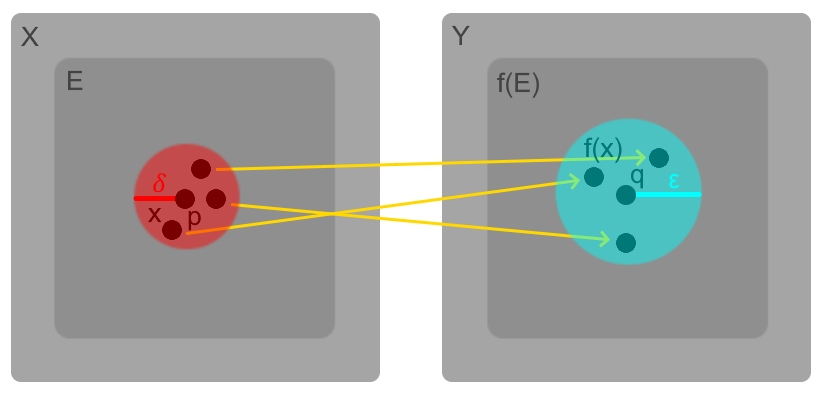
\includegraphics[scale=0.45]{Images/14.1.1.png}
\end{figure}

{ \color{red} Theorem 14.1.2:
Sequence definition of $\lim_{x \rightarrow p} f(x) = q$ }

    \begin{adjustbox}{minipage=14cm, right, vspace=0.1cm 0cm}
        $\lim_{x \rightarrow p} f(x) = q$ if and only if
        $\lim_{n \rightarrow \infty} f(p_n) = q$ for every
        sequence \{$p_n$\} $\in$ E where $p_n \not = p$ and
        $\lim_{n \rightarrow \infty} p_n = p$.
    \end{adjustbox}

{ \color{magenta} \underline{Proof} }

    \fbox{
    \begin{minipage}{15cm}
        Suppose $\lim_{x \rightarrow p} f(x) = q$.

        For $\epsilon$ $>$ 0, there is a $\delta$ $>$ 0 such that
        $d_Y(f(x),q) < \epsilon$ if x $\in$ E and $d_X(x,p) < \delta$.

        Choose \{$p_n$\} $\in$ E such that $p_n \not = p$
        and $\lim_{n \rightarrow \infty} p_n = p$.

        Then for $\delta > 0$, there is N such that for n $>$ N, then
        $d_X(p_n,p)< \delta$ so $d_Y(f(p_n),q) < \epsilon$.

        \vspace{0.2cm}

        Suppose $\lim_{x \rightarrow p} f(x) \not = q$.
        Then there is a $\epsilon$ $>$ 0 such that for every $\delta$ $>$ 0,
        there is a x $\in$ E where $d_Y(f(x),q) \geq \epsilon$, but
        $d_X(x,p) < \delta$.
        Let $\delta_n = \frac{1}{n}$ and thus, there is a \{$p_n$\}
        where $p_n \not = p$ and $\lim_{n \rightarrow \infty} p_n = p$,
        but $\lim_{n \rightarrow \infty} f(p_n) \not = q$.
    \end{minipage} }

    \vspace{0.5cm}

{ \color{orange} Corollary 14.1.3: A limit of a function is unique }

    \begin{adjustbox}{minipage=14cm, right, vspace=0.1cm 0cm}
        If f has a limit at p, this limit is unique.
    \end{adjustbox}

{ \color{magenta} \underline{Proof} }

    \fbox{
    \begin{minipage}{15cm}
        If $\lim_{x \rightarrow p} f(x) = q$, then by {\color{red} theorem 14.1.2},
        $\lim_{n \rightarrow \infty} f(p_n) = q$ for every
        \{$p_n$\} $\in$ E where $p_n \not = p$ and
        $\lim_{n \rightarrow \infty} p_n = p$.

        Thus, if there exists $\lim_{x \rightarrow p} f(x) = q'$, then there is
        a \{$p_n$\} $\in$ E where $p_n \not = p$ and
        $\lim_{n \rightarrow \infty} p_n = p$, but
        $\lim_{n \rightarrow \infty} f(p_n) = q'$ which is a contradiction.
    \end{minipage} }

    \vspace{0.5cm}

{ \color{red} Theorem 14.1.4: Arithemtic operations on functions of limits }

    \begin{adjustbox}{minipage=14cm, right, vspace=0.1cm 0cm}
        Let E $\subset$ X, p $\in$ E', and f(x),g(x) $\in$ $\mathbb{C}$ so 
        $\lim_{x \rightarrow p} f(x) = A$, $\lim_{x \rightarrow p} g(x) = B$.
    \end{adjustbox}

    \vspace{0.2cm}

    \begin{enumerate}[label=(\alph*), leftmargin=2cm, itemsep=0.1cm]
        \item $\lim_{x \rightarrow p} (f+g)(x) = A+B$
        \item $\lim_{x \rightarrow p} (fg)(x) = AB$
        \item $\lim_{x \rightarrow p} (\frac{f}{g})(x) = \frac{A}{B}$
    \end{enumerate}

\newpage





\subsection{ Continuous Functions }

{ \color{blue} Definition 14.2.1: Continuous functions on a set }

    \begin{adjustbox}{minipage=14cm, right, vspace=0.1cm 0cm}
        Suppose X,Y are metric spaces, E $\subset$ X, p $\in$ E, and
        f maps E into Y.

        f is continuous at p if:
        
        \begin{adjustbox}{minipage=13cm, right, vspace=0.1cm 0cm}
            For every $\epsilon > 0$, there is a
            $\delta > 0$ such that
            for all x $\in$ E
            
            where $d_X(x,p) < \delta$, then
            $d_Y(f(x),f(p)) < \epsilon$
        \end{adjustbox}

        f(p) have to be defined to be continuous.

        If f is continuous at every p $\in$ E, then f is continuous on E.

        f is continuous at isolated points since regardless of $\epsilon$,
        there is a $\delta > 0$ such that $d_X(x,p) < \delta$ is x = p so
        $d_Y(f(x),f(p)) = 0 < \epsilon$.
    \end{adjustbox}

\begin{figure}[h]
	\centering
	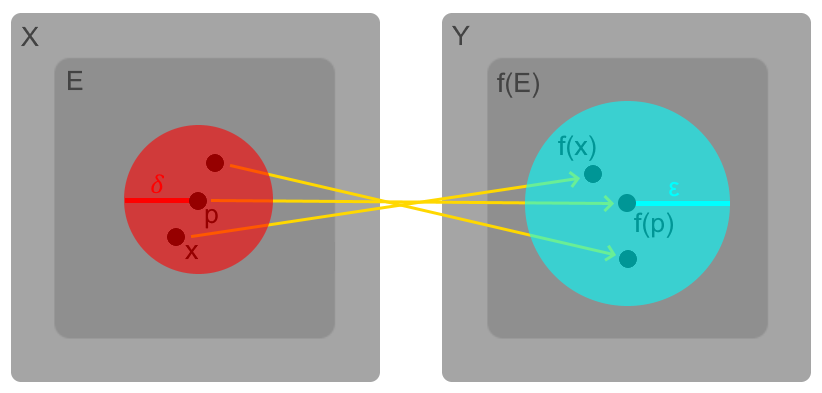
\includegraphics[scale=0.38]{Images/14.2.1.png}
\end{figure}

{ \color{red} Theorem 14.2.2: Continuity at p $\rightleftharpoons$ lim f(p) = f(p) }

    \begin{adjustbox}{minipage=14cm, right, vspace=0.1cm 0cm}
        Suppose E $\subset$ X, p $\in$ E, and
        f maps E into Y. Let p $\in$ E'.

        Then f is continuous at p if and only if
        $\lim_{x \rightarrow p} f(x) = f(p)$.
    \end{adjustbox}

{ \color{magenta} \underline{Proof} }

    \fbox{
    \begin{minipage}{15cm}
        If f is continuous at p, then for every $\epsilon > 0$, there
        is a $\delta > 0$ such that $d_Y(f(x),f(p)) < \epsilon$
        for all x $\in$ E where $d_X(x,p) < \delta$.
        Thus, $\lim_{x \rightarrow p} f(x) = f(p)$.

        \vspace{0.2cm}

        If $\lim_{x \rightarrow p} f(x) = f(p)$, then for every
        $\epsilon > 0$, there is a $\delta > 0$ where $d_Y(f(x),f(p)) < \epsilon$
        for all x $\in$ E where $d_X(x,p) < \delta$.
        Thus, f is continuous at p.
    \end{minipage} }

    \vspace{0.5cm}

{ \color{red} Theorem 14.2.3: Continuity Chain Rule }

    \begin{adjustbox}{minipage=14cm, right, vspace=0.1cm 0cm}
        Suppose E $\subset$ X, f: E $\rightarrow$ Y, g: f(E) $\rightarrow$ Z,
        and h: E $\rightarrow$ Z where h(x) = g(f(x)).

        If f is continuous at p and g is continuous at f(p),
        then h is continuous at p.
    \end{adjustbox}

{ \color{magenta} \underline{Proof} }

    \fbox{
    \begin{minipage}{15cm}
        Since g is continuous at f(p), then for $\epsilon > 0$, there is a
        $\delta_1$ such that:

        \hspace{1cm}
        $d_Z(g(y),g(f(p))) < \epsilon$ for $d_Y(y,f(p)) < \delta_1$
        where y $\in$ f(E)

        Since f is continuous at p, there is a $\delta_2 > 0$ such that:

        \hspace{1cm}
        $d_Y(f(x),f(p)) < \delta_1$ for $d_X(x,p) < \delta_2$ 
        where x $\in$ E

        Thus, $d_Z(h(x),h(p))$ = $d_Z(g(f(x)),g(f(p)))$ $<$ $\epsilon$
        for $d_X(x,p)$ $<$ $\delta_2$ where x $\in$ E.

        Thus, h is continuous at p.
    \end{minipage} }

\begin{figure}[h]
	\centering
	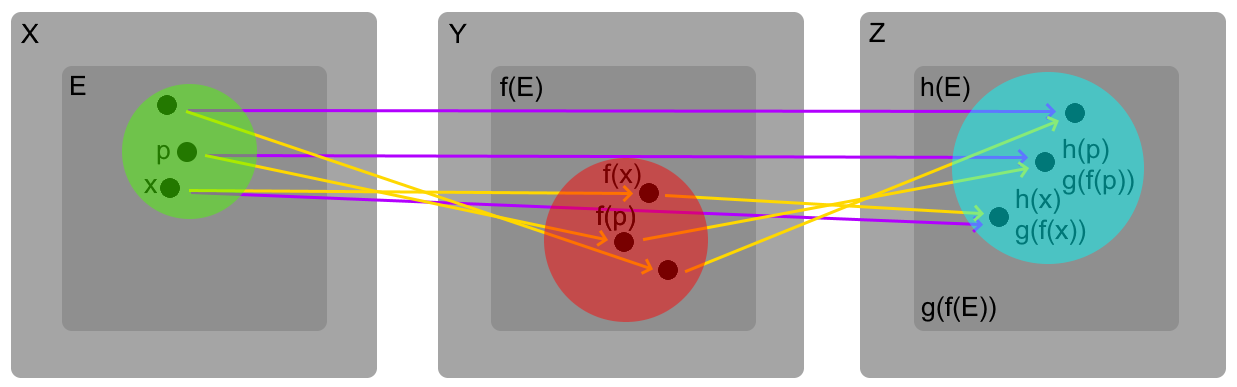
\includegraphics[scale=0.38]{Images/14.2.3.png}
\end{figure}

\newpage

{ \color{red} Theorem 14.2.4:
Continuous functions map open sets to open sets }

    \begin{adjustbox}{minipage=14cm, right, vspace=0.1cm 0cm}
        f: X $\rightarrow$ Y is continuous on X if and only if:

        \hspace{1cm}
        $f^{-1}(V)$ is open in X for every open set V in Y.
    \end{adjustbox}

{ \color{magenta} \underline{Proof} }

    \fbox{
    \begin{minipage}{15cm}
        Suppose f is continuous on X and V is an open set in Y.

        Suppose p $\in$ X and f(p) $\in$ V.
        Since V is open, there exists $\epsilon > 0$ such that
        y $\in$ V if $d_Y(y,f(p)) < \epsilon$.
        Since f is continuous at p, there exists $\delta > 0$ such that
        $d_Y(f(x),f(p)) < \epsilon$ for $d_X(x,p) < \delta$.
        Thus, x $\in$ $f^{-1}(V)$ for $d_X(x,p) < \delta$.

        \vspace{0.2cm}

        Suppose $f^{-1}(V)$ is open in X for every open V in Y.

        Fix p $\in$ X and $\epsilon > 0$.
        Let V be the set of all y $\in$ Y such that $d_Y(y,f(p)) < \epsilon$
        so V is open and thus, $f^{-1}(V)$ is open.
        Thus, there exists $\delta > 0$ such that x $\in$ $f^{-1}(V)$
        for $d_X(x,p) < \delta$.
        Since x $\in$ $f^{-1}(V)$, then f(x) $\in$ V so $d_Y(f(x),f(p)) < \epsilon$.
    \end{minipage} }

    \vspace{0.5cm}

{ \color{orange} Corollary 14.2.5:
Continuous functions map closed sets to closed sets }

    \begin{adjustbox}{minipage=14cm, right, vspace=0.1cm 0cm}
        f: X $\rightarrow$ Y is continuous on X if and only if:

        \hspace{1cm}
        $f^{-1}(C)$ is closed in X for every closed set C in Y.
    \end{adjustbox}

{ \color{magenta} \underline{Proof} }

    \fbox{
    \begin{minipage}{15cm}
        By {\color{red} theorem 14.2.4}, f is continuous
        if and only if $f^{-1}(V)$ is open in X for every open set V in Y.
        Let C = $V^c$.
        Since V is open, then C is closed.

        Since $f^{-1}(C)$
        = $f^{-1}(V^c)$
        = $(f^{-1}(V))^c$,
        then $f^{-1}(C)$ is closed since $f^{-1}(V)$ is open.
    \end{minipage} }

    \vspace{0.5cm}

{ \color{red} Theorem 14.2.6: Continuous functions }

    \begin{adjustbox}{minipage=14cm, right, vspace=0.1cm 0cm}
        Let f,g be complex continuous functions on X.

        Then f+g, fg, and $\frac{f}{g}$ where g $\not =$ 0 for all x $\in$ X
        are continuous on X.
    \end{adjustbox}

{ \color{magenta} \underline{Proof} }

    \fbox{
    \begin{minipage}{15cm}
        If x is an isolated point, f+g, fg, and $\frac{f}{g}$
        are continuous by definition.
        If x is a limit point, then by {\color{red} theorems 14.1.4 and 14.2.2},
        f+g, fg, and $\frac{f}{g}$ are continuous since

        \begin{itemize}[leftmargin=2cm, itemsep=0.1cm]
            \item $\lim_{x \rightarrow p} (f+g)(x)
                = \lim_{x \rightarrow p} f(x) + \lim_{x \rightarrow p} f(x)
                = f(p) + g(p)$
            \item $\lim_{x \rightarrow p} (fg)(x)
                = \lim_{x \rightarrow p} f(x) \lim_{x \rightarrow p} g(x)
                = f(p) g(p)$
            \item $\lim_{x \rightarrow p} (\frac{f}{g})(x)
                = \frac{\lim_{x \rightarrow p} f(x)}{\lim_{x \rightarrow p} g(x)}
                = \frac{f(p)}{g(p)}$
        \end{itemize}
    \end{minipage} }

    \vspace{0.5cm}

{ \color{red} Theorem 14.2.7: Continuous functions on $\mathbb{R}^k$ }

    \begin{enumerate}[label=(\alph*), leftmargin=1.5cm, itemsep=0.1cm]
        \item Let $f_1,...,f_k$: X $\rightarrow$ $\mathbb{R}$ and
        f: X $\rightarrow$ $\mathbb{R}^k$ where
        f(x) = ($f_1(x)$, ... , $f_k(x)$).

            Then f is continuous if and only if $f_1,...,f_k$ are continuous.

        \item If f and g are continuous mappings of X into $\mathbb{R}^k$,
        then f + g and f $\cdot$ g are continuous on X.
    \end{enumerate}

{ \color{magenta} \underline{Proof} }

    \fbox{
    \begin{minipage}{15cm}
        Since $|f_i(x) - f_i(y)|$
        $\leq$ $\sqrt{\sum_1^k |f_i(x) - f_i(y)|^2}$
        = $|f(x) - f(y)|$, then if f is continuous, then
        each $f_i$ is continuous and vice versa.

        \vspace{0.2cm}

        Since f,g are continuous, then by part a, each $f_i$,$g_i$ are continuous.
        Then by {\color{red} theorem 14.2.6},
        each $f_i + g_i$ and $f_i g_i$ are continuous so
        by part a, f + g and f $\cdot$ g are continuous.

        \vspace{0.2cm}

        Thus, every polynomial, rational, and absolute value function is continuous
        since polynomials are $x_1 \cdot ... \cdot x_k$ where each $x_i$
        is continuous, rationals are polynomials divided by polynomials,
        and $||x| - |y|| \leq |x - y|$ implies $|x|$ is continuous.
    \end{minipage} }




